\documentclass[xcolor=pdftex,dvipsnames,table,mathserif]{beamer}
\usetheme{default}
%\usetheme{Darmstadt}
%\usepackage{times}
%\usefonttheme{structurebold}

\usepackage[english]{babel}
%\usepackage[table]{xcolor}
\usepackage{pgf,pgfarrows,pgfnodes,pgfautomata,pgfheaps}
\usepackage{amsmath,amssymb,setspace,centernot}
\usepackage[latin1]{inputenc}
\usepackage[T1]{fontenc}
\usepackage{relsize}
\usepackage{pdfpages}
\usepackage[absolute,overlay]{textpos} 


\newenvironment{reference}[2]{% 
  \begin{textblock*}{\textwidth}(#1,#2) 
      \footnotesize\it\bgroup\color{red!50!black}}{\egroup\end{textblock*}} 

\DeclareMathSizes{10}{10}{6}{6} 

\begin{document}
\title{Part 6: Duration Analysis}
\author{Chris Conlon}
\institute{Microeconometrics}
\date{\today}

\frame{\titlepage}

\section{Intro}

\begin{frame}
\frametitle{Overview}
Another way to look at dynamic behavior
\begin{itemize}
\item In the previous lecture we looked a single agent dynamics where optimizing agents made decisions over multiple periods.
\item The maintained assumption in that case was that $F(X' | X)$ was a 1st order Markov Process and was exogenous to the agent's decision and we treated it like a \alert{nuisance parameter}.
\item Sometimes the object of interest is actually the \alert{transition function} itself.
\item We are often interested in the length of \alert{spells} or how much time is spent in each state which we call \alert{duration}.
\end{itemize}
\end{frame}

\begin{frame}
\frametitle{Overview}
Simple cases:
\begin{itemize}
\item The simplest cases are single irreversible transitions
\begin{itemize}
\item Alive $\rightarrow$ Dead
\item Working $\rightarrow$ Failure
\end{itemize}
\item Other easy cases are ``resetting'' processes:
\begin{itemize}
\item Employed $\rightarrow$ unemployed for zero weeks, one week, etc.
\item Healthy $\rightarrow$ Sick Day 1, Sick Day 2, etc.
\item Not on strike $\rightarrow$ Strike Day 1, Strike Day 2, etc.
\end{itemize}
\item Let's start with these before we worry about multivariate outcomes or more complicated cases.
\end{itemize}
\end{frame}


\begin{frame}
\frametitle{Decisions}
Have to make some decisions first
\begin{enumerate}
\item Do we model \alert{spell length} directly or \alert{probability of transition}?
\begin{itemize}
\item Most of the time we want to work with probability of transition.
\item If we work with probability of transition, we have to pay attention to \alert{frequency}
\end{itemize}
\item What outcomes do we measure: \alert{stocks}? or \alert{flows}?
\begin{itemize}
\item Do we measure the number of people who lose/find jobs?
\item Do we measure the number of unemployed people each month?
\end{itemize}
\item Is the data \alert{truncated} or \alert{censored}?
\begin{itemize}
\item People who are still alive are not in the dataset!
\end{itemize}
\end{enumerate}
For now we will think about \alert{single-spells}, and measure them using \alert{flow data}.
\end{frame}

\begin{frame}
\frametitle{Examples}
There are lots of different names (depending on your discipline):
\begin{itemize}
\item Life table analysis
\item Hazard Analysis
\item transition analysis
\item survival analysis
\item failure time analysis
\end{itemize}
Examples:
\begin{itemize}
\item How long does a government last?
\item How long does a part last?
\item How long before a firm adopts a new technology?
\item How long do marriages last?
\item How long before criminals re-offend?
\end{itemize}
\end{frame}

\begin{frame}
\frametitle{Start with a Graph!}
\begin{center}
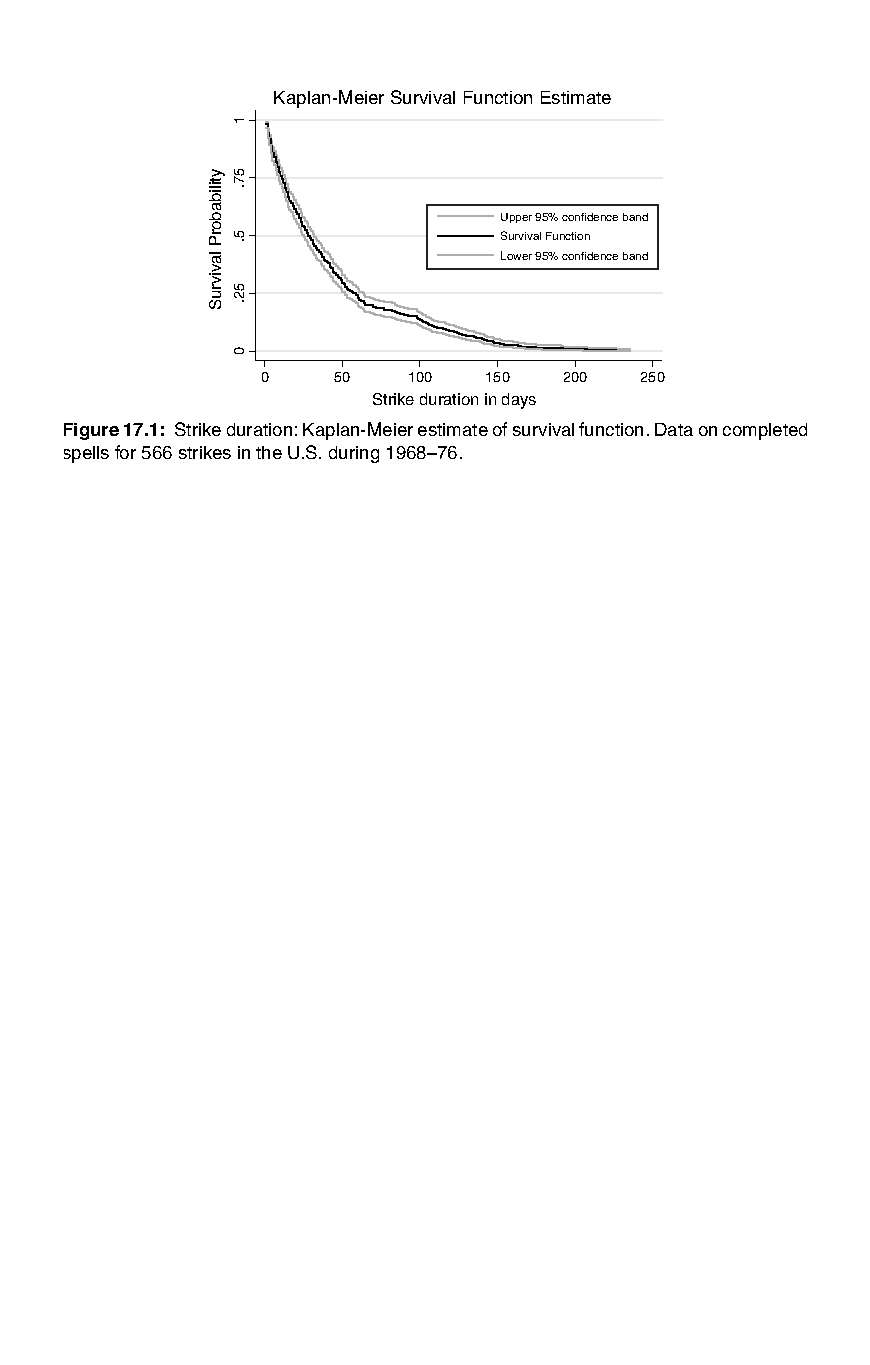
\includegraphics[width=4.5in]{./resources/figure17-1.pdf}
\end{center}
\end{frame}

\begin{frame}
\frametitle{What did we just plot?}
The \alert{empirical survival function}
\begin{itemize}
\item We ignored any covariates, including calendar time.
\item The x-axis was the duration
\item The y-axis was the fraction of observations still alive ``alive'' after $x$ periods.
\item If nothing is infinitely lived then the graph always starts at $1$ and always ends at zero.
\item If things are infinitely lived we call the duration distribution \alert{defective}.
\end{itemize}
\end{frame}

\begin{frame}
\frametitle{Parametric}
Let's start with some deeply parametric stuff
\begin{itemize}
\item density function: $f(t) = d F(t) / dt$: unconditional probability of instantaneous failure
\item CDF: $F(t) = Pr(T \leq t) = \int_0^{\infty} f(s) d s$. (Probability that spell is less than length $t$).
\item Survival Function: $S(t) = 1- F(t) = Pr( T > t)$. This has the nice property that it integrates to expected duration $\int_0^{\infty} S(t) d t = E[T]$.
\item Hazard Function: $\lambda(t)  = \lim_{\Delta t \rightarrow 0} \frac{Pr[t \leq T < t+ \Delta t | T \geq t]}{\Delta t} = \frac{f(t)}{S(t)}$.
\item \alert{All of these functions represent the same information!}
\end{itemize}
\end{frame}

\begin{frame}
\frametitle{More about hazard functions}
\begin{itemize}
\item Hazard is conditional probability of leaving unemployment after being unemployed for $t$.
\item Hazard is percentage change in survivor function $S(t)$
\item Hazard also gives us the distribution of duration $T$:
\begin{eqnarray*}
\lambda(t) &=& - \frac{\partial \log S(t)}{\partial t}\\
S(t) &=& \exp \left[ - \int_0^{\infty} \lambda(u) d u \right]
\end{eqnarray*}
\item Often we'd like to estimate $\lambda(t | x)$ instead of $E[T | x]$ especially since we often have \alert{censored} data so that  $\lambda(t | x)$ is still well defined but $E[T | x]$ is not.
\item In practice  $\lambda(t | x)$ can be tricky to estimate (especially since it may contain zeros at some $t$ in finite sample. Solution: \alert{Cumulative Hazard Function}.
\begin{eqnarray*}
\Lambda(t) = \int_0^{\infty} \lambda(s) d s = - \log S(t)
\end{eqnarray*}
\item Just like we preferred to estimate CDF instead of PDF!
\end{itemize}
\end{frame}

\begin{frame}
\frametitle{Summary Table}
\begin{center}
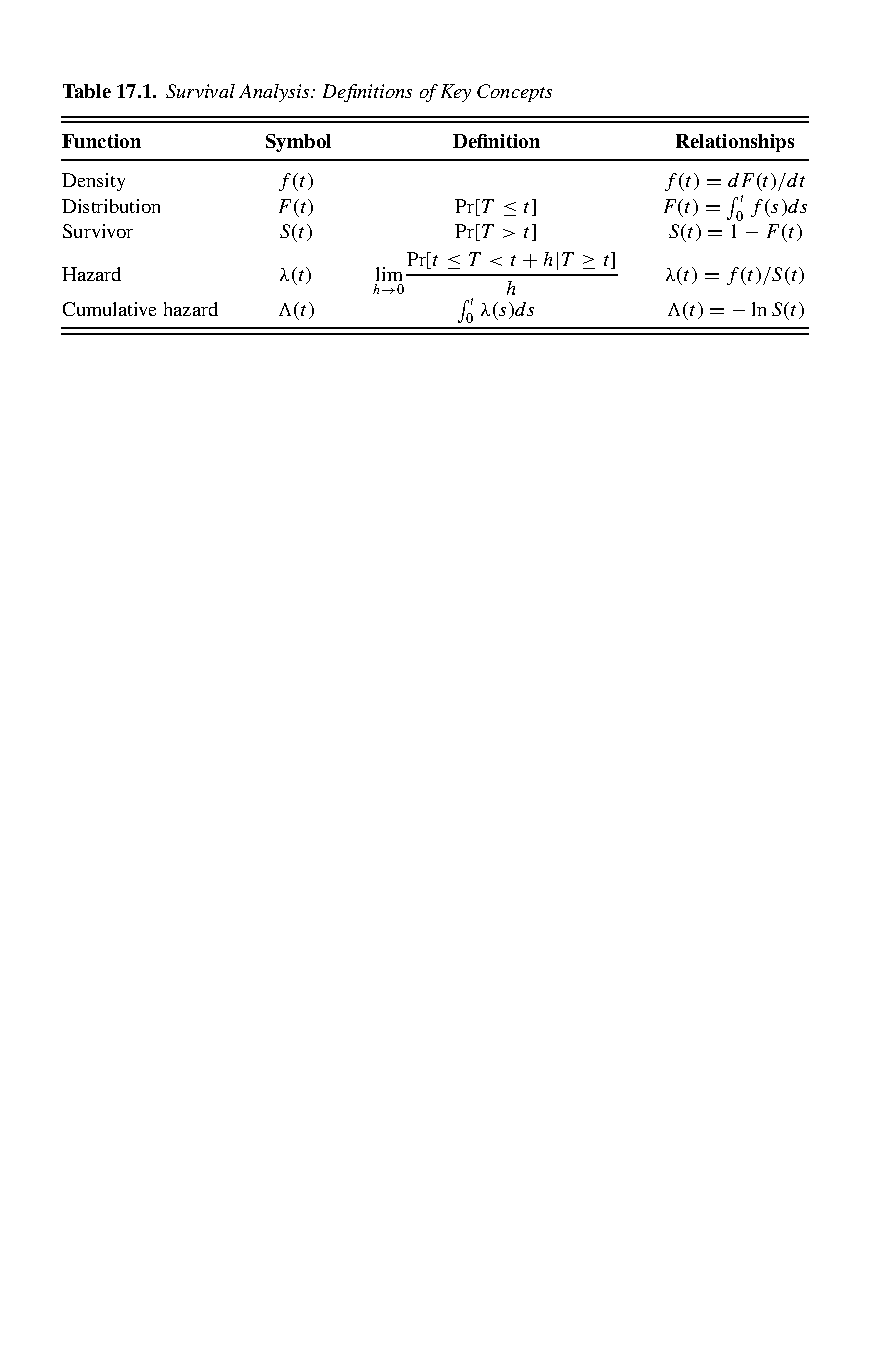
\includegraphics[width=4.5in]{./resources/parametrictable1.pdf}
\end{center}
\end{frame}

\begin{frame}
\frametitle{What about Discrete Time?}
\begin{itemize}
\item Maybe we only see survival annually/weekly/etc. not actual failure time.
\item Basic idea is the same. Have to be careful about ties. Divide failures into $t_j$ buckets
\begin{eqnarray*}
\lambda_j &=& Pr[T = t_j | T \geq t_j] = f^d(t_j) / S^d(t_{j-})\\
\Lambda^d(t)&=&\sum_{j | t_j \leq t} \lambda_j \\
S^d &=& Pr [T \geq t ] = \prod_{j| t_j \leq t} (1-\lambda_j)
\end{eqnarray*}
\item Can define the \alert{product integral} which is regular product in discrete case and exponential of integral in continuous case.
\end{itemize}
\end{frame}



\begin{frame}
\frametitle{Nonparametric estimation}
\begin{itemize}

\item Without censoring, things are easy: just let
\[
\hat{S}(t)=\frac{1}{n}\sum_{i=1}^n \mathbf{1} (T_i \geq  t).
\]
\item if you want a smooth hazard function, take a smooth estimator, e.g.
(with some ``small'' bandwidth $w>0$)
\[
\hat{S}(t)=\frac{1}{n}\sum_{i=1}^n \frac{1}{1+\exp((t-T_i)/w)},
\]
\item and then take minus the derivative of the log of this estimate.
\end{itemize}
\alert {What if there is censoring?} Kaplan-Meier!
\end{frame}



\begin{frame}
\frametitle{Censoring}
Lots of ways for censoring to arise:
\begin{itemize}
\item Mostly concerned about \alert{right censoring} 
\item Observe spells from time $0$ until time $c$ and all we know is that they end in $(c,\infty)$.
\end{itemize}
\end{frame}


\begin{frame}
\frametitle{Kaplan-Meier}
\begin{itemize}
\item We define the
ordered durations as 
\[
T_{(1)} < \ldots < T_{(n)},
\]
\item let $d_j$ be the number of observations $i$ for which $T_i=T_{(j)}$
\item Let $m_j$ number of spels censored in $[t_j,t_{j+1})$
\item and $r_j$ the cardinality of the \alert{risk set}  at duration $t_{j-}$   $r_j=\sum_{l | l \geq j} d_l + m_l$
\item Simple estimate of the hazard function $\hat{\lambda}_j = \frac{d_j}{r_j}$.
\item Kaplan-Meier estimator  of the survival function is the \alert{Product Limit Estimator}
\[
\hat{S}(t)=\Pi_{j|t_j \leq t} \left(
1-\frac{d_j}{r_j}
\right) = \Pi_{j|t_j \leq t} \left(
\frac{r_j- d_j}{r_j}
\right)
\]
\item It is normally distributed (asymptotically), with (Greenwood) variance
\[
\hat{V}[\hat{S}(t)]=(\hat{S}(t))^2 \cdot \sum_{j|t_j \leq t}
\frac{d_j}{r_j(r_j-d_j)}.
\]
\end{itemize}
\end{frame}

\begin{frame}
\frametitle{Other stuff}
Think about what happens when $m_j= 0$ (no censoring)
\begin{itemize}
\item $r_j=\sum_{l | l \geq j} d_l + m_l \rightarrow r_{j+1} = r_j - d_j$.
\item $ \hat{S}(t)= \Pi_{j|t_j \leq t} \left( \frac{r_j- d_j}{r_j} \right) =  \Pi_{j|t_j \leq t} \frac{r_{j+1}}{r_j} = \frac{r_j}{N}$
\item Again -- exactly what we would expect -- one minus the ECDF.
\end{itemize}
How do we deal with ties?
\begin{itemize}
\item Lots of ties can create problems. Implicitly we assume all deaths are at same time in period.
\item Why does this matter-- well how many are remaining in $r_j$?
\item $r_j$ is potentially biased if we have lots of ties.
\item Can either try corrections or sample data at higher frequency
\end{itemize}
\end{frame}




\begin{frame}
\frametitle{Parametric models}
 Usually we specify directly the hazard function (closer to theory).
\begin{itemize}
\item \emph{Economic example:\/} an unemployed person ($T \geq t$)  leaves unemployment
when (given that his benefits decrease in time) he has an offer with a wage $w \geq r(t)$, a reservation wage
\item wage offers arrive with some probability $p_t$, and a distribution such that
$\Pr(w\geq s)=\bar{G}_t(s)$.
\item Then someone unemployed at $t$ leaves unemployment at $t$   with probability 
$p_t \bar{G}_t(r(t))$
so the hazard function is 
\[ 
\lambda(t)=p_t\bar{G}_t(r(t)).
\]
\item A job search model would give us a theory for $r(.)$, $p_t$  and $\bar{G}_t$,
 up to some parameters to be estimated, and conditional on covariates $x$.
\end{itemize}
\end{frame}

\begin{frame}
\frametitle{Exponential and Weibull }
\begin{itemize}
\item The exponential is popular because it has a \alert{constant hazard rate} $\lambda(t) =\gamma$ which does not depend on $t$.
\item This is often referred to as the \alert{memorylessness} property of the exponential.
\item This is analytically convenient but it makes it hard to fit things in practice (you only have one parameter!)
\item The Weibull is a generalization with $\lambda(t) = \gamma \alpha t^{\alpha-1}$. For $\alpha=1$ we have exponential.
\item For $\alpha > 1$ i is increasing and for $\alpha < 1$ it is decreasing (monotonically). 
\item Weibull used to be popular in econometrics for simple parametric analysis.
\end{itemize}
\end{frame}


\begin{frame}
\frametitle{Exponential and Weibull }
\begin{center}
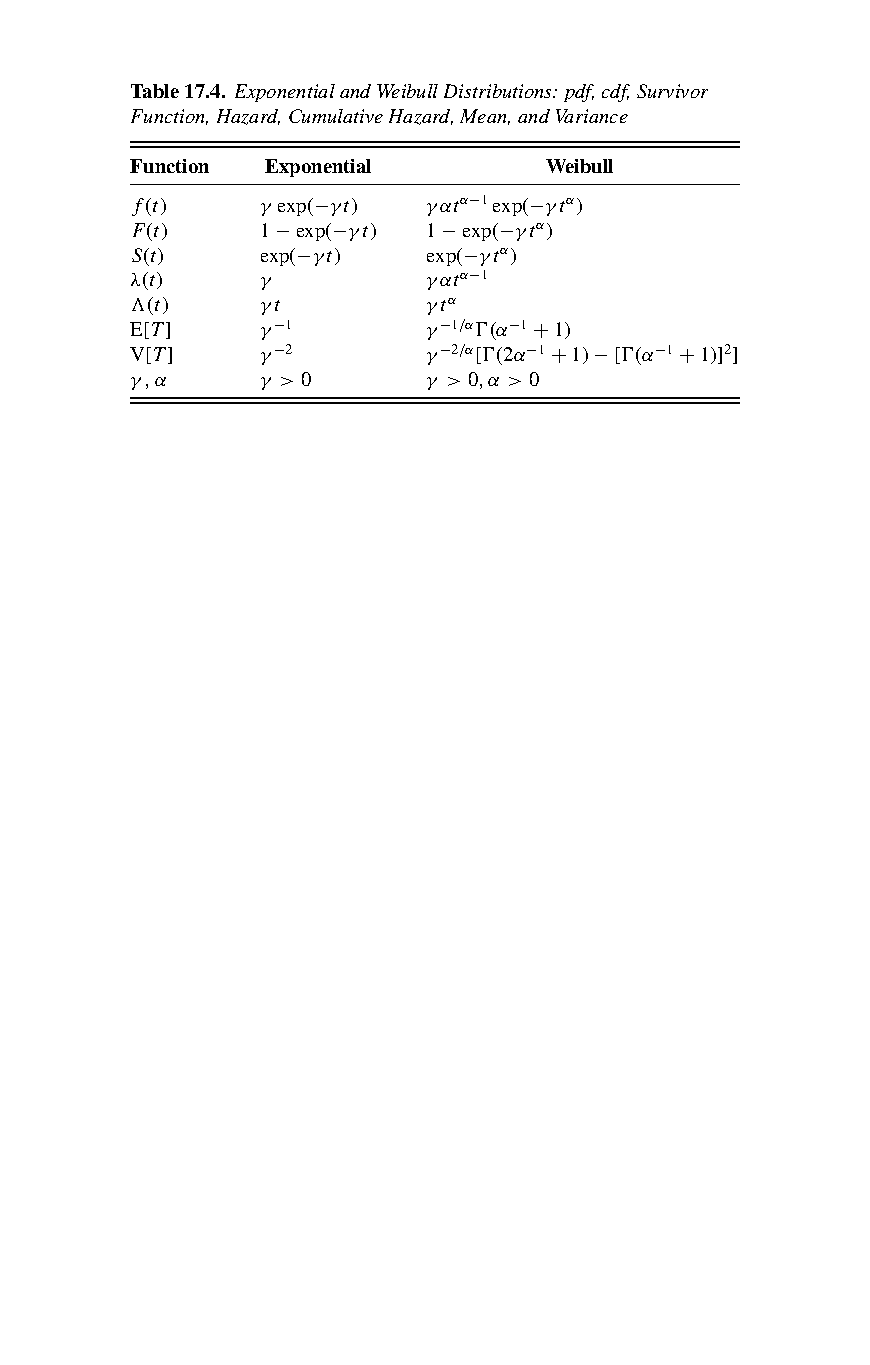
\includegraphics[width=4.5in]{./resources/figure17-4.pdf}
\end{center}
\end{frame}


\begin{frame}
\frametitle{Comparison of Parametric Models}
\begin{center}
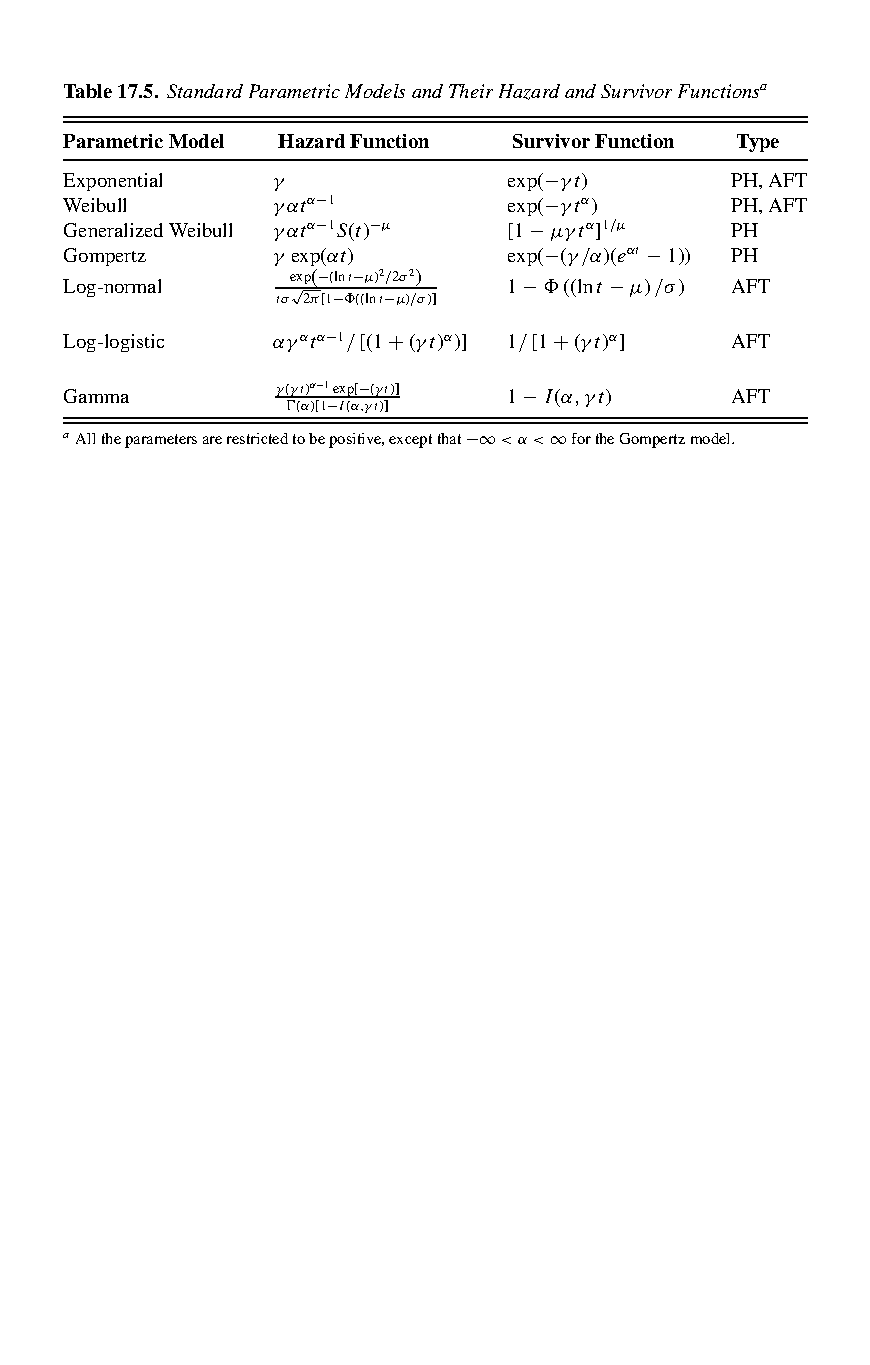
\includegraphics[width=4.5in]{./resources/figure17-5.pdf}
\end{center}
\end{frame}

\begin{frame}
\frametitle{Adding Covariates }
\begin{itemize}
\item We can also add covariates by letting $\gamma = \beta X$.
\item Sometimes this is called \alert{link function} or \alert{generalized linear models} similar to what we saw with the logit or probit.
\item It is usually a bad idea to link more than one nonlinear parameter this way.
\item We would typically estimate via MLE. Writing down the full-data log-likelihood is straightforward.
\item A frequently used special-case are \alert{proportional hazard models}
\end{itemize}
\end{frame}




\begin{frame}
\frametitle{The Proportional Hazard  Model}
With covariates $x$, the hazard function is $h(t \vert x)$; we specify
\[
\lambda(t \vert x)=\lambda_0(t)\phi(x).
\]
\begin{itemize}
\item $\lambda_0$ and $\phi$ are up to a positive multiplicative constant.)
\item  We call $\lambda_0$ the \alert{ baseline hazard}; every individual has
a hazard that is just a proportional version of the baseline hazard.
\end{itemize}
The baseline hazard could be:
\begin{itemize}
\item constant: the survival function is exponential
\item a power function $\lambda_0(t)=\gamma t^{\alpha}$; e.g. for
$\alpha<0 $ we have \alert{negative duration dependence} (the
long-term unemployed\ldots)
\item more complicated (flexible) specifications.
\end{itemize}
\end{frame}



\begin{frame}
\frametitle{Estimating the PH Model}
{\bf Maximum likelihood:} works for any parametric modelx
$\lambda(t \vert x,\beta)$ of the full hazard function;\\
(here: w/o censoring, without corrleation across individuals):
\[
\max_{\beta} \sum_{i=1}^n \ln f(T_i \vert x_i,\beta),
\]
where $f(t \vert x,\beta)$ is the density of the duration $T$ induced by
$\lambda$:
\[
f(t \vert x)=\lambda(t \vert x)S(t \vert x)=\lambda(t \vert x)\exp(-\Lambda(t \vert x)),
\]
so the log-likelihood for $i$ is just $\ln
\lambda(T_i \vert x_i,\beta)-\Lambda(T_i \vert x_i,\beta)$.
\end{frame}

\begin{frame}
\frametitle{What's the point?}
\begin{itemize}
\item The (partial) additive separability of the log-likelihood in the PH model is designed to make our lives easier.
\item Presumably, we specified $\lambda$ so that its integral $\Lambda$ is easy to
compute. 
\item For PH: the log-likelihood for $i$ is:\\
$\ln \lambda_0(T_i,\beta)+\ln\phi(x_i,\beta)-\Lambda_0(T_i,\beta)\phi(x_i,\beta)$.
\item The most common choice is $\phi(x_i,\beta) = \exp(x_i \beta)$ so that $\ln\phi(x_i,\beta) = x_i \beta$.
\item In that case we have that $\partial \lambda/ \partial x_j = \beta_j \cdot \lambda$.
\item One remaing problem: what to do with the baseline hazard function (is that even identified?).
\end{itemize}
\end{frame}

\begin{frame}
\frametitle{Cox's Partial Likelihood for the PH Model}
\begin{itemize}
\item if we do not want to assume anything about the shape of the \alert{baseline hazard function}
\item but we are happy specifying $\phi(x,\beta)$
\item then we will only look at the {\em order\/} of the durations: we
reorder individuals so that $T_{i_1}<\ldots<T_{i_n}$
\item \ldots and we forget about the durations! Then the partial
likelihood is:
\[
\sum_{j=1}^n
\left(
 \ln \phi(x_{i_j},\beta)
  -\ln
  \left(
  \sum_{l=j}^n
\phi(x_{i_l},\beta)
\right)
\right).
\]
\item This is a \alert{limited information maximum likelihood estimator}. It is not fully efficient!
\item But it may be robust to mis-specifying $\lambda_0$.  Is it actually a valid likelihood? \alert{not sure!}.
\end{itemize}
\end{frame}

\begin{frame}
\frametitle{How did that work?}
Once we have ordered everything:
\begin{itemize}
\item Let $R(t_j)$ be the set of spells at risk (still alive) at $t_j$
\item $d_j$ are the deaths at time $t_j$ $\sum_l \mathbf{1}[t_l = t_j]$.
\item Consider only at-risk spells ending a fixed $t_j$
\begin{eqnarray*}
Pr[T_j = t_j \vert R(t_j)] &=& \frac{Pr[T_j = t_j \vert T_j \geq t_j]}{\sum_{l \in R(t_j)} Pr[T_l = t_l \vert T_l \geq t_j]}\\
 &=& \frac{\lambda_j(t_j | x_j, \beta) ]}{\sum_{l \in R(t_j)} \lambda_l (t_j,x_l,\beta)}\\
 &=& \frac{\phi( x_j, \beta) }{\sum_{l \in R(t_j)} \phi (x_l,\beta)}\\
\end{eqnarray*}
\item $\lambda_0$ drops out because of PH.
\end{itemize}
\end{frame}

\begin{frame} 
\frametitle{Why?}
\begin{itemize}
\item \emph{Intuition:\/} those individuals who exit first are (on average) those in
the risk set whose covariates $x$ give them the largest $\phi(x,\beta)$.
\item After we have $\hat{\beta}$ we can estimate the baseline integrated
hazard; denoting $N(t)$=number of individuals with $T=t$
\[
\widehat{\Lambda_0}(T_{i_j})=\sum_{m=1}^j \frac{N(T_{i_m})}{\sum_{l=m}^n
\phi(x_{i_l},\hat{\beta})}.
\]
\end{itemize}
\end{frame}


\begin{frame}
\frametitle{Tricks}

{\em A simple way to test the model}:
\begin{itemize}
\item just take two different groups of individuals, estimate PH on each, check whether the baseline
hazards look \alert{proportional} \textbf{NOT} \alert{equal}
\end{itemize}

 {\em testing a  parametric specification of the baseline
hazard $\bar{\Lambda}_0$:} 
\begin{itemize}
\item define  generalized residuals $\bar{u}_i=\bar{\Lambda_0}(T_i)$
\item Under the true  model, for any $z$
\[
\Pr(\bar{u} <z) \simeq
\Pr(T_i<\bar{\Lambda}_0^{-1}(z))=1-S_0(\bar{\Lambda}_0^{-1}(z)).
 \]
\item it should be $1-\exp(-z)$ if $S_0=\exp(-\bar{\Lambda}_0)$.
\item So you can estimate the integrated hazard of
 $(\bar{u}_1,\ldots,\bar{u}_n)$; it should be $\Lambda_u(z) \equiv z$.
\end{itemize}
\end{frame}


\begin{frame}
\frametitle{The PH Model is Usually too Restrictive}
\begin{itemize}
\item {\bf Fact:}  the hazard rate of leaving unemployment decreases
in time;
\item It could be {\em skimming}: the more able, more willing, better
connected find a job faster;
\item or it could be ``technological'': skills deteriorate over time.
\item Under the PH model it can only be the latter: negative duration
dependence. $\rightarrow$ introduce unobserved heterogeneity:
\[
\lambda(t \vert x,v)=\lambda_0(t)\phi(x) v.
\]
\item $v$ is a ``type'' that is unobserved by the econometrician; we
only assume that it is uncorrelated with $x$ and independent of $t$.
\end{itemize}
\end{frame}

 \begin{frame}
 \frametitle{Dynamic selection}
\begin{itemize}
\item The model with $v$ is called the \textbf{Mixed PH model} (MPH).
\item In the unemployment story: the larger $v$'s have a higher hazard
  rate, so they find a job faster
\item Over time, the distribution of $v$ moves (stochastically) to the
  left.
\item This \alert{dynamic selection} is a general phenomenon in the MPH
  model: $\lambda(t \vert x)$ has ``more negative duration dependence'' than
  $\lambda(t \vert x,v)$.
\item Can we test dynamic selection vs true negative duration dependence
  ($\lambda_0$ decreasing)? $\rightarrow$ identification issues.
  \item This idea shows up in dynamic models of durable goods purchases as well.
  \end{itemize}
\end{frame}



\begin{frame}
\frametitle{Identification}
We still can recover the aggregate survival function from the data, but now it
is a mixture:
\[
S^A(t \vert x)=\Pr(T \geq t \vert x)=
\int \exp(-v \phi(x)\Lambda_0(t))dF(v).
\]
\begin{itemize}
\item Can we recover $\phi$ and $\lambda_0$ without assuming anything on $F$?
\item Almost \ldots\ in theory: we just need to assume that $E(v)$ is finite.
\end{itemize}
\end{frame}



\begin{frame}
\frametitle{A Constructive Proof, 1}
\begin{itemize}
\item Normalize $Ev=1$; and $\phi(x_0)=1$ for some $x_0$. 
\item Then the aggregate hazard function is
\[
\lambda^A(t \vert x)=-\frac{\partial \log S^A}{\partial t}(t \vert x)
\]
that is
\[
\frac{\int v \phi(x)\lambda_0(t)\exp(-v \phi(x)\Lambda_0(t))dF(v)}{S^A(t \vert x)}.
\]
\item
Look at $x=x_0$ and $t=0^+$: then $\Lambda_0(t) \simeq 0$, so
\[
\lambda^A(0^+\vert x_0)=\frac{Ev \times k(x_0) \times \lambda_0(0)}{S^A(0\vert x_0)}=\lambda_0(0).
\]
\item
and
\[
\phi(x)=\frac{\lambda^A(0^+ \vert x)}{\lambda^A(0^+ \vert x_0)}.
\]
\end{itemize}
\end{frame}

\begin{frame}
\frametitle{A Constructive Proof, 2}
\begin{itemize}
\item Now we can define
\[
m^A(t \vert x)=-\frac{\partial \log S^A(t,x)}{\partial \phi(x)}
\]
\item and we get the baseline hazard from 
\[
\frac{\lambda_0(t)}{\Lambda_0(t)}=\frac{\lambda^A(t \vert x)}{m^A(t \vert x)};
\]
\item  and we can also recover $F$. 
\item In practice we would specify functional forms of course.
\end{itemize}
\end{frame}


\begin{frame}
\frametitle{Is that Practical?}
\begin{itemize}
\item We are relying heavily on ``identification at 0'': that is where we
get $\phi(x)$, the rest depends on it.
\item Empirical researchers have found that it is often a slim basis (and a
very slow-converging estimator)---but
anything else will be parametric.
\item The alternative is to use richer data: multiple durations/multiple spells. 
\end{itemize}
\end{frame}

\begin{frame}
\frametitle{Application 1: job search}
E.g. Cahuc/Postel-Vinay-Robin, {\em Econometrica \/} 2006.
\begin{itemize}
\item Workers are heterogeneous, so are firms; 
\item a worker quits when he gets a better outside offer (exogenous Poisson($\lambda$)).
\item We observe (given matched employer-employee data): 
\begin{itemize}
\item job durations (how long each worker stays in a job)
\item and distributions of wages (mostly) across firms.
\end{itemize}
\end{itemize}
\end{frame}


\begin{frame}
\frametitle{Bad luck}
\begin{itemize}
\item The likelihood for the duration of job spells is independent of heterogeneity!
\[
f(t)=\frac{\delta(\delta+\lambda)}{\lambda}\int_{\delta t}^{(\delta+\lambda)t} \frac{\exp(-x)}{x} dx.
\]
\item So we can identify $\lambda$ and $\delta$, and nothing about heterogeneity of firms and workers.
\item (But the good thing is that we don't need to assume anything about it and we get $\delta$ and $\lambda$).
\end{itemize}
\end{frame}

\begin{frame}
\frametitle{Better luck}
\begin{itemize}
\item Given bargaining on wages, outside options matter;
\item and outside options generate option values, which increase with heterogeneity ( volatility!).
\item ``So'' by looking at the distribution of wages we can infer heterogeneity.
\end{itemize}
\end{frame}


\begin{frame}
\frametitle{Application 2: moral hazard in insurance}
Abbring-Chiappori-Pinquet, {\em JEEA\/} 2003.
\begin{itemize}
\item Insurees have exogenous  types (risk) $v$ that are unobserved; we call this adverse selection;
\item they also decide to adopt a risky behavior or not: \alert{moral hazard}.
\item Data typically gives us a series of claims for each individual. 
\item A state could be: ``I have had exactly $p$ claims so far'' and a spell is the time between two claims.
\end{itemize}
\end{frame}


\begin{frame}
\frametitle{Duration dependence}
\begin{itemize}
\item Adverse selection induces positive duration dependence: the time between claims is positively correlated.
\item On the other hand, with experience rating a claim (at fault) increases premia and makes risky behavior more costly---typically
\item so moral hazard induces negative duration dependence.
\item How can we test for the latter while controlling for the former?
\end{itemize}
\end{frame}


\begin{frame}
\frametitle{The Model}
\begin{itemize}
\item The hazard function for claim $(p+1)$ at $t$, given state $p$, is (dropping $x$)
\[
v h_0(t) A^{-p},
\]
\item  with $A$ and $h_0$ unknown. 
\item $v$ models exogeneous unobserved risk, 
\item every time a claim occurs, the hazard for the next claim is divided by  $A$: moral hazard.
\item It is the MPH, with a twist: the $p$.
\end{itemize}
\end{frame}


\begin{frame}
\frametitle{Estimating Finite Mixtures}
\begin{itemize}
\item In practice estimating finite mixture models can be tricky.
\item A simple example is the mixture of normals (incomplete data likelihood)
\begin{eqnarray*}
f(x_1,\ldots,x_n | \theta) = \prod_{i=1}^N \sum_{k=1}^K \pi_k f(x_i | \mu_k, \sigma_k)
\end{eqnarray*}
\item We need to find both mixture weights $\pi_k = Pr(z_k)$ and the components $(\mu_k,\sigma_k)$ the weights define a valid probabiltiy measure $\sum_k \pi_k = 1$.
\item Easy problem is \alert{label switching}. Usually it helps to order the components by say decreasing $\pi_1 > \pi_2 > \ldots$ or  $\mu_1 > \mu_2 > \ldots$ 
\item The real problem is that which component you belong to is unobserved. We can add an extra indicator variable $z_{ik} \in \{0,1\}$.
\item We don't care about $z_{ik}$ per-se so they are \alert{nuisance parameters}.
\end{itemize}
\end{frame}

\begin{frame}
\frametitle{Estimating Finite Mixtures}
\begin{itemize}
\item We can write the complete data log-likelihood (as if we observed $z_{ik}$):
\begin{eqnarray*}
l(x_1,\ldots,x_n | \theta) = \sum_{i=1}^N  \log \left( \sum_{k=1}^K I[z_i = k]  \pi_k f(x_i \mu_k, \sigma_k) \right)
\end{eqnarray*}
\item We can instead maximized the expected log-likelihood where we take the expectation $E_{z|\theta}$
\begin{eqnarray*}
\alpha_{ik}(\theta) = Pr(z_{ik} =1 | x_i,\theta) = \frac{f_k(x_i,z_k,\mu_k,\sigma_k) \pi_k }{\sum_{m=1}^K f_m(x_i,z_m,\mu_m,\sigma_m) \pi_m}
\end{eqnarray*}
\item Now we have a probability $\hat{\alpha}_{ik}$ that gives us the probability that $i$ came from component $k$. We also compute $\hat{\pi}_k = \frac{1}{N} \sum_{i=1}^N \alpha_{ik}$
\end{itemize}
\end{frame}

\begin{frame}
\frametitle{EM Algorithm}
\begin{itemize}
\item Treat the $\hat{\alpha}_k(\theta^{(q)})$ as data and maximize to find $\mu_k,\sigma_k$ for each $k$
\begin{eqnarray*}
\hat{\theta}^{(q+1)} = \arg \max_{\theta}  \sum_{i=1}^N  \log \left( \sum_{k=1}^K \hat{\alpha}_k(\theta^{(q)}) f(x_i | z_{ik}, \theta ) \right)
\end{eqnarray*}
\item We iterate between updating $\hat{\alpha}_k(\theta^{(q)})$ (E-step) and $\hat{\theta}^{(q+1)}$ (M-step)
\item For the mixture of normals we can compute the M-step very easily:
\begin{eqnarray*}
\mu_k^{(q+1)} &=& \frac{1}{N} \sum_{i=1}^N \hat{\alpha}_k(\theta^{(q)}) x_{i}\\
\sigma_k^{(q+1)} &=& \frac{1}{N} \sum_{i=1}^N \hat{\alpha}_k(\theta^{(q)}) (x_{i} - \overline{x})^2 \\
\end{eqnarray*}
\end{itemize}
\end{frame}

\begin{frame}
\frametitle{EM Algorithm}
\begin{itemize}
\item EM algorithm has the advantage that it avoids complicated integrals in computing the expected log-likelihood over the missing data.
\item For a large set of families it is proven to converge to the MLE
\item That convergence is \alert{monotonic} and \alert{linear}. (Newton's method is quadratic)
\item This means it can be slow, but sometimes $\nabla_{\theta} f (\cdot)$ is really complicated.
\end{itemize}
\end{frame}

\begin{frame}
\frametitle{My own example: Conlon Mortimer: AEJ 2013}
\begin{itemize}
\item Probability of sales of $j$ depend on the set of available products $a_t$ some $x$'s (supressed) and some unknown parameters $\theta$ so that $p_j(a_t,\theta)$
\item Imagine a multinomial logit with random coefficients
\item At the beginning of the day/week we observe $a_t$. 
\item At some point during the week a product $k$ stocked out such that $a_t' = a_t \setminus k$.
\item BUT we dont know which sales happened before or after the stockout.
\item Now the probability of a sale is given by: $\lambda p_j(a_t,\theta) + (1-\lambda) p_j(a_t',\theta)$ where $\lambda$ is the fraction of consumers who arrive before the stockout.
\end{itemize}
\end{frame}

\begin{frame}
\frametitle{My own example: Conlon Mortimer: AEJ 2013}
\begin{itemize}
\item Again we don't observe $(y_{jt}^0,y_{jt}^1)$ (sales before or after the stockout)
\item However we do see the total sales $y_{jt} = y_{jt}^0+ y_{jt}^1$
\item And we know something about product $k$ (the one that stocks out)
\item We know that $y_{kt}^{1} = 0$ by definition!
\item We can compute the distribution of $f(\lambda | \theta, y_{kt})$ (when did the stockout occur?)
\end{itemize}
\end{frame}

\begin{frame}
\frametitle{My own example: Conlon Mortimer: AEJ 2013}
What is $f(\lambda | \theta, y_{kt})$?
\begin{itemize}
\item How many consumers arrived before $y_{kt}$ consumers purchased good $k$?
\item If sales are binomial then this is given by a \alert{negative binomial} distribution. This is an example of a \alert{hititng process} or \alert{discrete duration model}.
\item Now I can compute 
\begin{eqnarray*}
\hat{y}_{jt}^{0} &=&y_{jt} \int \frac{\lambda p_j(a_t,\theta)}{\lambda p_j(a_t,\theta) +(1-\lambda)\cdot p_j(a_t',\theta)} f(\lambda | \theta, y_{kt}) d \lambda \\
\hat{y}_{jt}^{1} &=&y_{jt} -\hat{y}_{jt}^{0} 
\end{eqnarray*}
\item The M-step is just our usual MLE for logit, nested-logit, rc-logit treating $\hat{y}_{jt}$ as data.
\end{itemize}
\end{frame}

\begin{frame}
\frametitle{My own example: Conlon Mortimer: AEJ 2013}
What was the point?
\begin{itemize}
\item We found that biases were large!
\item Goods that stocked out a lot we understated demand for!
\item Goods that were net recipients of substitution we overstated demand for!
\item Basically you should pay attention to which other products are available.
\end{itemize}
\end{frame}







\end{document}
